\section{Público objetivo}
    La audiencia objetivo de este proyecto se enfoca principalmente en los usuarios finales, pero también incluye a las entidades administrativas y a sus trabajadores que se beneficiarán de este sistema.

    Los usuarios finales son los colectivos más afectados por la brecha digital, principalmente las personas con falta de competencias digitales o sin acceso a la tecnología.
    En particular, los principales beneficiarios serán las personas mayores, que suelen presentar mayores dificultades con la tecnología, especialmente en lo respectivo a la realización de trámites administrativos online.
    Aunque también, podrán verse favorecidos otros colectivos vulnerables de este sistema, como personas con discapacidades físicas o cognitivas que les dificulten el uso de dispositivos tecnológicos, personas con bajos recursos económicos que no puedan permitirse las tecnologías, personas que vivan en zonas rurales o aisladas de la conexión a la red.
        
    Por otro lado, las entidades administrativas también forman parte de la audiencia objetivo, ya que se ven beneficiadas de la automatización de los trámites, reduciendo la carga de trabajo de sus empleados y liberándolos de tareas más engorrosas. 
    Al disponer de una línea telefónica atendida por inteligencia artificial, los empleados pueden dejar de atender multitud de peticiones diarias y liberar tiempo para otras tareas. Además, con la ayuda de la plataforma web administrativa, pueden gestionar y supervisar las solicitudes de una manera eficiente.
        
    Por último, cualquier persona fuera de estas características puede utilizar el sistema sin ningún problema, en caso de que no tengan un ordenador a mano o que simplemente les resulte más cómodo para ahorrar tiempo.
        
\section{Alcance del sistema}
    El proyecto contempla el desarrollo de un sistema de gestión de trámites administrativos simulado capaz de hacer una representación fiel de la implementación futura real. 
    Para ello se han definido unos límites, quedando incluidos en el alcance del proyecto los siguientes aspectos:
    \begin{itemize}
        \item La gestión de trámites administrativos de organismos públicos, limitados a la provincia de Valladolid, con el fin de acotar el desarrollo, evitando una generalización excesiva que dificulte la implementación del prototipo y manteniendo la representatividad del sistema.
        \item Una plataforma web limitada a la administración y supervisión de los empleados, los trámites y las solicitudes realizadas a través del sistema.
        \item Un sistema de llamadas VoIP para la iniciación y recepción de llamadas, que simule la red telefónica.
        \item Un agente conversacional de inteligencia artificial capaz de informar y recopilar los datos necesarios de los trámites seleccionados.
    \end{itemize}
    Y quedando fuera del alcance del proyecto los siguientes aspectos:
    \begin{itemize}
        \item La integración con sistemas reales de las Administraciones públicas, ya que el objetivo es simular con datos ficticios el inicio y cómo se llevaría a cabo el trámite, pero no se pretende completar ningún proceso real.
        \item El uso del agente de inteligencia artificial para otros fines distintos a la gestión de los trámites seleccionados.
        \item La utilización de la infraestructura de telefonía tradicional, dado que una solución VoIP reduce los costes asociados al uso y alquiler de líneas y ofrece una experiencia de interacción equivalente para el usuario.
        \item El proyecto contempla solo fases de desarrollo y pruebas; no entra en el alcance del proyecto fases de producción, envío real de correos electrónicos ni la publicación de la plataforma web.
    \end{itemize}
        
    \subsection{Trámites}
        La selección de los trámites incluidos en el sistema es uno de los pasos fundamentales en el análisis, ya que determina el realismo del sistema. 
        La importancia recae en incorporar distintos tipos de gestiones de diferentes organizaciones que incluyan distintos tipos de cumplimiento, de tal forma que la simulación sea variada y representativa. 
            
        Además, no sirve con elegir cualquier trámite, tienen que ser de valor para las personas objetivo, ofreciéndoles una alternativa útil que vayan a utilizar frente a las otras soluciones existentes.
        Los trámites seleccionados son los siguientes:
        \begin{itemize}
            \item Trámite 1. Solicitud del certificado de empadronamiento en el ayuntamiento de Valladolid. 
                Este documento es necesario para la realización de otros trámites, como la solicitud de ayudas o beneficios exclusivos para residentes locales. 
                Es una gestión factible que se realiza online mediante un formulario, frente a la alternativa de acudir al ayuntamiento presencialmente para obtenerlo. 
            \item Trámite 2. Solicitar una cita en la Agencia Tributaria en la provincia de Valladolid. 
                Aunque ya se ha comentado que hay algunas Administraciones que ya implementan bots de llamadas para solicitar citas previas, esta tecnología los mejora. 
                Para nuestro sistema simulado nos vamos a centrar en la AEAT ya que ofrece servicios de valor para el público objetivo, y la cita telefónica que disponen actualmente solo es atendida por personal durante unas horas concretas. 
                Con esta implementación se ampliaría el soporte a cualquier hora y día y se liberaría trabajo a los operadores de la agencia.
            \item Trámite 3. Solicitar la tarjeta sanitaria de SACYL por pérdida o robo en la provincia de Valladolid. 
                Este procedimiento cumple también con los requisitos de ser un trámite útil, ya que, el usuario objetivo requiere de los servicios de salud pública con mayor frecuencia y la tarjeta sanitaria es necesaria para acceder a estos servicios. 
                Además, se realiza también mediante un formulario en línea, evitando la necesidad de acudir presencialmente al centro de salud, evitando desplazamientos y esperas innecesarias.
        \end{itemize}
            
\section{Requisitos}
    A continuación, se elicitan los requisitos funcionales, no funcionales y de información que debe cumplir el sistema:
    \begin{enumerate}
        \item[RF1.] El sistema deberá permitir a los usuarios finales interaccionar con él a través de una conversación telefónica.
        \item[RF2.] El usuario podrá solicitar su certificado de empadronamiento de la ciudad de Valladolid.
        \item[RF3.] El usuario podrá reservar una cita en la agencia tributaria para la provincia de Valladolid.
        \item[RF4.] El usuario podrá obtener su tarjeta sanitaria de SACYL en caso de pérdida o robo en la provincia de Valladolid.
        \item[RF5.] El sistema deberá permitir a los empleados identificarse con su usuario y contraseña en la plataforma web administrativa.
        \item[RF6.] El sistema deberá limitar las funcionalidades de la aplicación web en función del rol del empleado (administrador o secretario).
        \item[RF7.] El sistema deberá almacenar todas las peticiones registradas a través de la IA.
        \item[RF8.] El sistema mostrará a los empleados un listado con todas las peticiones del sistema y permitirá seleccionarlas individualmente para mostrar información de esa petición concreta.
        \item[RF9.] El sistema deberá permitir a los secretarios de la Administración correspondiente asignarse y resolver manualmente las peticiones revisables que requieran asistencia humana.
        \item[RF10.] El sistema deberá permitir a los secretarios crear una petición manualmente en la página web con el objetivo de subsanar situaciones excepcionales derivadas de errores humanos o fallos del sistema.
        \item[RF11.] El sistema deberá permitir a los administradores añadir otros empleados al sistema.
        \item[RF12.] El sistema mostrará a los administradores una lista con los empleados registrados en el sistema, permitiendo desactivarlos o modificar su información.
        \item[RF13.] El sistema deberá permitir a los administradores añadir trámites al sistema.
        \item[RF14.] El sistema mostrará a los administradores una lista con los trámites del sistema, permitiendo desactivarlos o modificar su información.
        \item[RF15.] El sistema permitirá a los empleados consultar su información personal y modificar su contraseña.
        
        \item[RFI1.] El sistema deberá almacenar la siguiente información con respecto a las peticiones:
            \begin{itemize}
                \item ID (identificador único de cada petición)
                \item Tipo (Trámite 1, 2 o 3)
                \item Teléfono (número del llamante)
                \item Información (datos extraídos por la IA en la llamada) 
                \item Estado (creada, pendiente, asignada, modificada, completada o cancelada)
                \item Fecha de creación
                \item Fecha de modificación (empleado que se asignó la tarea)
            \end{itemize}
        \item[RFI2.] El sistema deberá almacenar la siguiente información con respecto a los empleados:
            \begin{itemize}
                \item Usuario
                \item Contraseña
                \item Nombre
                \item Primer apellido
                \item Segundo apellido
                \item Email
                \item Rol (administrador o secretario)
                \item Foto de perfil
                \item Estado (activo o inactivo)
            \end{itemize}
        \item[RFI3.] El sistema deberá almacenar la siguiente información con respecto a los trámites:
            \begin{itemize}
                \item ID (identificador único de cada trámite)
                \item Nombre del trámite
                \item Estado (activo o inactivo)
            \end{itemize}
                
        \item[RNF1.] Los errores registrados por la IA, por falta de comprensión o entrenamiento, no deben superar el 10\% de las peticiones.
        \item[RNF2.] El tiempo de respuesta del agente conversacional en llamada no debe superar los 3 segundos para dar sensación de fluidez en la conversación.
        \item[RNF3.] La interfaz de la web de empleados será intuitiva y fácil de usar, de forma que el 95\% de los empleados puedan completar tareas clave con menos de 2 errores y en menos de 5 minutos por tarea.
    \end{enumerate}

\section{Casos de uso}
    \subsection{Diagrama de casos de uso:}
        \begin{figure}[H]
            \centering
            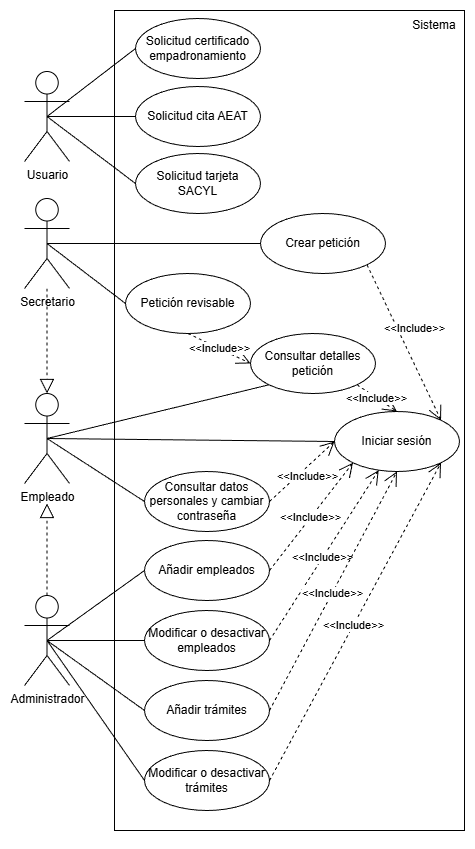
\includegraphics[width=0.6\textwidth]{img/diagramas/diagrama_casos_uso.png}
            \caption{Diagrama de casos de uso.}
        \end{figure}

    \subsection{Actores:}
        \begin{enumerate}
            \item Usuario: persona ajena a la Administración pública que necesita un servicio de la misma.
                Se comunica con el sistema mediante llamadas telefónicas.
            \item Empleados: representa a un trabajador de los organismos públicos. 
                Tienen acceso a la web interna y desempeñan distintas acciones en función de su rol. 
                \begin{itemize}
                    \item Administrador: su función principal es la gestión de empleados y trámites en la plataforma interna.
                    \item Secretario: se encargan de supervisar y completar las peticiones. 
                        También pueden crear peticiones manualmente en caso de que sea necesario, ya sea por subsanar algún error o por cualquier otra razón. 
                \end{itemize}
        \end{enumerate}

    \subsection{Solicitud del certificado de empadronamiento:}
        \begin{longtable}{|p{16cm}|} 
        \hline
        \textbf{Solicitud del certificado de empadronamiento} \\ \hline
        \textbf{Actor principal:} Usuario \\ \hline
        \textbf{Precondición:} El usuario ha iniciado la llamada al sistema \\ \hline
        \textbf{Secuencia normal:} \\
        \begin{minipage}[t]{\linewidth}
            \begin{enumerate}
                \item El usuario solicita obtener el certificado de empadronamiento.
                \item El sistema solicita el DNI.
                \item El usuario proporciona el DNI.
                \item El sistema solicita el nombre.
                \item El usuario proporciona su nombre.
                \item El sistema solicita los dos apellidos.
                \item El usuario proporciona sus dos apellidos.
                \item El sistema solicita el teléfono.
                \item El usuario proporciona su teléfono.
                \item El sistema solicita el motivo de la petición.
                \item El usuario responde el motivo de la petición.
                \item El sistema repite la información obtenida y solicita confirmación. 
                \item El usuario confirma los datos.
                \item El sistema almacena la petición.
                \item El sistema rellena el formulario de solicitud del certificado de empadronamiento con los datos obtenidos.
            \end{enumerate}
            \vspace{1mm}
        \end{minipage} \\ \hline
        \textbf{Flujos alternativos:} \\
        \begin{minipage}[t]{\linewidth}
            \begin{enumerate}
                \item[11.a] Si el usuario no confirma los datos, el sistema repite las preguntas correspondientes y se continúa con el paso siguiente a la pregunta.
            \end{enumerate}
            \vspace{1mm}
        \end{minipage}\\ \hline
        \caption{Descripción general del caso de uso - Solicitud del certificado de empadronamiento.}
        \end{longtable}
        
    \subsection{Solicitud de cita en la Agencia Tributaria:}
        \begin{longtable}{|p{16cm}|} 
        \hline
        \textbf{Solicitud de cita en la Agencia Tributaria} \\ \hline
        \textbf{Actor principal:} Usuario. \\ \hline
        \textbf{Precondición:} El usuario ha iniciado una llamada al sistema. \\ \hline
        \textbf{Secuencia normal:}\\
        \begin{minipage}[t]{\linewidth}
            \begin{enumerate}
                \item El usuario solicita agendar una cita en la Agencia Tributaria.
                \item El sistema solicita el DNI.
                \item El usuario proporciona su DNI.
                \item El sistema solicita el nombre y el primer apellido.
                \item El usuario proporciona su nombre y sus primer apellido.
                \item El sistema solicita el tipo de servicio.
                \item El usuario proporciona el tipo de servicio.
                \item El sistema pregunta si prefiere cita telefónica o presencial.
                \item El usuario responde que presencial.
                \item El sistema solicita la oficina.
                \item El usuario responde la oficina.
                \item El sistema solicita fecha y hora preferible para la cita.
                \item El usuario responde la fecha y hora.
                \item El sistema comprueba que la fecha y hora es válida.
                \item El sistema repite la información obtenida y solicita confirmación. 
                \item El usuario confirma los datos.
                \item El sistema almacena la petición.
                \item El sistema rellena el formulario para agendar la cita.
            \end{enumerate} 
            \vspace{1mm}
        \end{minipage} \\ \hline
        \textbf{Flujos alternativos:} \\
        \begin{minipage}[t]{\linewidth}
            \begin{enumerate}
                \item[9.a.] Si el usuario responde cita telefónica se continúa con el paso 15.
                \item[14.a.] Si la fecha u hora no es válida se vuelve al paso 12.
                \item[16.a] Si el usuario no confirma los datos, el sistema repite las preguntas correspondientes y se continúa con el paso siguiente a la pregunta.
            \end{enumerate}
            \vspace{1mm}
        \end{minipage} \\ \hline
        \caption{Descripción general del caso de uso - Solicitud de cita en la Agencia Tributaria.}
        \end{longtable}
        
    \subsection{Solicitud de la tarjeta sanitaria de SACYL por pérdida o robo:}
        \begin{longtable}{|p{16cm}|} 
        \hline
        \textbf{Solicitud de la tarjeta sanitaria de SACYL por pérdida o robo} \\ \hline
        \textbf{Actor principal:} Usuario. \\ \hline
        \textbf{Precondición:} el usuario ha iniciado una llamada al sistema. \\ \hline
        \textbf{Secuencia normal:} \\
        \begin{minipage}[t]{\linewidth}
            \begin{enumerate}
                \item El usuario solicita la tarjeta sanitaria.
                \item El sistema solicita el motivo (pérdida o robo).
                \item El usuario proporciona el motivo (pérdida o robo).
                \item El sistema solicita el nombre.
                \item El usuario proporciona su nombre.
                \item El sistema solicita el primer apellido.
                \item El usuario proporciona su primer apellido.
                \item El sistema solicita la fecha de nacimiento.
                \item El usuario proporciona su fecha de nacimiento.
                \item El sistema pregunta el centro de salud.
                \item El usuario responde su centro de salud.
                \item El sistema solicita la dirección.
                \item El usuario responde la dirección.
                \item El sistema repite la información obtenida y solicita confirmación. 
                \item El usuario confirma los datos.
                \item El sistema almacena la petición.
                \item El sistema rellena el formulario para solicitar la tarjeta sanitaria.
            \end{enumerate}
            \vspace{1mm}
        \end{minipage} \\ \hline
        \textbf{Flujos alternativos:} \\
        \begin{minipage}[t]{\linewidth}
            \begin{enumerate}
                \item[15.a] Si el usuario no confirma los datos, el sistema repite las preguntas correspondientes y se continúa con el paso siguiente a la pregunta.
            \end{enumerate}
            \vspace{1mm}
        \end{minipage} \\ \hline
        \caption{Descripción general del caso de uso - Solicitud de la tarjeta sanitaria de SACYL por pérdida o robo.}
        \end{longtable}

    \subsection{Iniciar sesión:}
    \label{subsec:2.4.5.}
        \begin{longtable}{|p{16cm}|} 
        \hline
        \textbf{Iniciar sesión} \\ \hline
        \textbf{Actor principal:} Empleado. \\ \hline
        \textbf{Secuencia normal:} \\
        \begin{minipage}[t]{\linewidth}
            \begin{enumerate}
                \item El sistema solicita el usuario o correo electrónico y la contraseña.
                \item El empleado introduce su usuario o correo electrónico y su contraseña.
                \item El sistema comprueba que los datos coinciden con un empleado e inicia sesión.
            \end{enumerate}
            \vspace{1mm}
        \end{minipage} \\ \hline
        \textbf{Flujos alternativos:} \\
        \begin{minipage}[t]{\linewidth}
            \begin{enumerate}
                \item[3.a.] Si los datos no coinciden con un empleado, el sistema informa de datos incorrectos y vuelve al paso 1.
                \item[3.b.] Si los datos coinciden pero el ususario está desactivado, el sistema lo informa y vuelve al paso 1.
            \end{enumerate}
            \vspace{1mm}
        \end{minipage} \\ \hline
        \textbf{Postcondiciones:} el empleado está identificado en el sistema. \\ \hline
        \caption{Descripción general del caso de uso - Iniciar sesión.}
        \end{longtable}

    \subsection{Consultar detalles de una petición:}
    \label{subsec:2.4.6.}
        \begin{longtable}{|p{16cm}|} 
        \hline
        \textbf{Consultar detalles de una petición} \\ \hline
        \textbf{Actor principal:} Empleado. \\ \hline
        \textbf{Precondición:} caso de uso \hyperref[subsec:2.4.5.]{2.4.5. Inicia sesión}. \\ \hline
        \textbf{Secuencia normal:} \\
        \begin{minipage}[t]{\linewidth}
            \begin{enumerate}
                \item El empleado va a la página con la lista de peticiones.
                \item El empleado clica en el ID de la petición.
                \item El sistema muestra la información de la petición.
            \end{enumerate}
            \vspace{1mm}
        \end{minipage} \\ \hline
        \caption{Descripción general del caso de uso - Consultar detalles de una petición.}
        \end{longtable}

    \subsection{Petición revisable:}
        \begin{longtable}{|p{16cm}|} 
        \hline
        \textbf{Petición revisable} \\ \hline
        \textbf{Actor principal:} Secretario. \\ \hline
        \textbf{Precondición:} caso de uso \hyperref[subsec:2.4.6.]{2.4.6. Consultar detalles de una petición}. \\ \hline
        \textbf{Secuencia normal:} \\
        \begin{minipage}[t]{\linewidth}
            \begin{enumerate}
                \item El secretario se asigna la petición.
                \item El secretario modifica la información necesaria.
                \item El secretario completa la petición.
                \item El sistema inicia el trámite correspondiente a la petición.
                \item El sistema actualiza el estado de la petición a completada. 
            \end{enumerate}
            \vspace{1mm}
        \end{minipage} \\ \hline
        \textbf{Flujos alternativos:} \\
        \begin{minipage}[t]{\linewidth}
            \begin{enumerate}
                \item[3.a.] Si el secretario anula la petición, cambia y actualiza el estado a cancelada y finaliza el caso de uso. 
            \end{enumerate}
            \vspace{1mm}
        \end{minipage} \\ \hline
        \caption{Descripción general del caso de uso - Petición revisable.}
        \end{longtable}

    \subsection{Consultar datos personales y cambiar contraseña:}
        \begin{longtable}{|p{16cm}|} 
        \hline
        \textbf{Consultar datos personales y cambiar contraseña} \\ \hline
        \textbf{Actor principal:} Empleado. \\ \hline
        \textbf{Precondición:} caso de uso \hyperref[subsec:2.4.5.]{2.4.5. Inicia sesión}. \\ \hline
        \textbf{Secuencia normal:} \\
        \begin{minipage}[t]{\linewidth}
            \begin{enumerate}
                \item El empleado clica en su perfil.
                \item El sistema muestra su información personal.
                \item El empleado clica en cambiar contraseña.
                \item El sistema solicita la contraseña actual y la contraseña nueva.
                \item El empleado introduce la información.
                \item El sistema comprueba que la contraseña actual es verídica.
                \item El sistema actualiza la contraseña del empleado.
            \end{enumerate}
            \vspace{1mm}
        \end{minipage} \\ \hline
        \textbf{Flujos alternativos:} \\
        \begin{minipage}[t]{\linewidth}
            \begin{enumerate}
                \item[6.a.] Si la contraseña actual es incorrecta, el sistema lo informa y vuelve al paso 4.
            \end{enumerate}
            \vspace{1mm}
        \end{minipage} \\ \hline
        \caption{Descripción general del caso de uso - Consultar datos personales y cambiar contraseña.}
        \end{longtable}

    \subsection{Crear petición:}
        \begin{longtable}{|p{16cm}|} 
        \hline
        \textbf{Crear petición} \\ \hline
        \textbf{Actor principal:} Secretario. \\ \hline
        \textbf{Precondición:} caso de uso \hyperref[subsec:2.4.5.]{2.4.5. Inicia sesión}. \\ \hline
        \textbf{Secuencia normal:} \\
        \begin{minipage}[t]{\linewidth}
            \begin{enumerate}
                \item El secretario va a la página con la lista de peticiones.
                \item El secretario clica en crear petición.
                \item El sistema solicita el teléfono y el trámite.
                \item El secretario introduce el teléfono y el trámite.
                \item El sistema solicita la información correspondiente al trámite.
                \item El secretario introduce la información.
                \item El sistema crea la petición e inicia el trámite.
            \end{enumerate}
            \vspace{1mm}
        \end{minipage} \\ \hline
        \caption{Descripción general del caso de uso - Crear petición.}
        \end{longtable}

    \subsection{Añadir empleados:}
        \begin{longtable}{|p{16cm}|} 
        \hline
        \textbf{Añadir empleados} \\ \hline
        \textbf{Actor principal:} Administrador. \\ \hline
        \textbf{Precondición:} caso de uso \hyperref[subsec:2.4.5.]{2.4.5. Inicia sesión}. \\ \hline
        \textbf{Secuencia normal:} \\
        \begin{minipage}[t]{\linewidth}
            \begin{enumerate}
                \item El administrador va a la página con la lista de empleados.
                \item El administrador selecciona añadir empleado.
                \item El sistema solicita los datos del nuevo empleado.
                \item El administrador rellena los datos.
                \item El sistema comprueba que el email no está registrado ya en el sistema.
                \item El sistema crea un usuario y una contraseña temporal.
                \item El sistema envía al nuevo usuario su contraseña temporal.
                \item El sistema almacena el nuevo empleado.
            \end{enumerate}
            \vspace{1mm}
        \end{minipage} \\ \hline
        \textbf{Flujos alternativos:} \\
        \begin{minipage}[t]{\linewidth}
            \begin{enumerate}
                \item[5.a.] Si el email ya está registrado, el sistema lo informa y continúa con el paso 3.
            \end{enumerate}
            \vspace{1mm}
        \end{minipage} \\ \hline
        \caption{Descripción general del caso de uso - Añadir empleados.}
        \end{longtable}

    \subsection{Modificar o desactivar empleados}
        \begin{longtable}{|p{16cm}|} 
        \hline
        \textbf{Modificar o desactivar empleados} \\ \hline
        \textbf{Actor principal:} Administrador. \\ \hline
        \textbf{Precondición:} caso de uso \hyperref[subsec:2.4.5.]{2.4.5. Inicia sesión}. \\ \hline
        \textbf{Secuencia normal:} \\
        \begin{minipage}[t]{\linewidth}
            \begin{enumerate}
                \item El administrador va a la página con la lista de empleados.
                \item El administrador clica en el botón de la columna activo del empleado correspondiente.
                \item El sistema muestra los campos con la información del empleado.
                \item El administrador modifica la información correspondiente y clica en editar.
                \item El sistema actualiza la información del empleado.
            \end{enumerate}
            \vspace{1mm}
        \end{minipage} \\ \hline
        \textbf{Flujos alternativos:} \\
        \begin{minipage}[t]{\linewidth}
            \begin{enumerate}
                \item[3.a.] El administrador clica en resetear contraseña, el sistema crea una contraseña temporal y se la envía al email del empleado.
                \item[4.a.] El administrador modifica el email, el sistema comprueba que el email ya está registrado en el sistema, lo informa y vuelve al paso 3.
                \item[4.b.] El administrador modifica el email, el sistema comprueba que el email no está registrado en el sistema y continúa con el paso 5.
                \item[4.c.] El administrador activa o desactiva el empleado, el sistema se lo avisa al email del empleado y continúa en el paso 5.
            \end{enumerate}
            \vspace{1mm}
        \end{minipage} \\ \hline
        \caption{Descripción general del caso de uso - Modificar o desactivar empleados.}
        \end{longtable}

    \subsection{Añadir trámites:}
        \begin{longtable}{|p{16cm}|} 
        \hline
        \textbf{Añadir trámites} \\ \hline
        \textbf{Actor principal:} Administrador. \\ \hline
        \textbf{Precondición:} caso de uso \hyperref[subsec:2.4.5.]{2.4.5. Inicia sesión}. \\ \hline
        \textbf{Secuencia normal:} \\
        \begin{minipage}[t]{\linewidth}
            \begin{enumerate}
                \item El administrador va a la página con la lista de trámites.
                \item El administrador clica en añadir trámite.
                \item El sistema solicita el nombre y estado del trámite.
                \item El administrador introduce el nombre y estado del trámite.
                \item El sistema comprueba que no hay otro trámite con el mismo nombre.
                \item El sistema actualiza los datos del trámite.
            \end{enumerate}
            \vspace{1mm}
        \end{minipage} \\ \hline
        \textbf{Flujos alternativos:} \\
        \begin{minipage}[t]{\linewidth}
            \begin{enumerate}
                \item[5.a.] El sistema comprueba que hay otro trámite con el mismo nombre, lo informa y vuelve al paso 3.
            \end{enumerate}
            \vspace{1mm}
        \end{minipage} \\ \hline
        \caption{Descripción general del caso de uso - Añadir trámites.}
        \end{longtable}

    \subsection{Modificar o desactivar trámites:}
        \begin{longtable}{|p{16cm}|} 
        \hline
        \textbf{Modificar o desactivar trámites} \\ \hline
        \textbf{Actor principal:} Administrador. \\ \hline
        \textbf{Precondición:} caso de uso \hyperref[subsec:2.4.5.]{2.4.5. Inicia sesión}. \\ \hline
        \textbf{Secuencia normal:} \\
        \begin{minipage}[t]{\linewidth}
            \begin{enumerate}
                \item El administrador va a la página con la lista de trámites.
                \item El administrador clica en el botón de la columna activo del trámite correspondiente.
                \item El sistema muestra los campos con la información del trámite.
                \item El administrador modifica la información correspondiente y clica en editar.
                \item El sistema actualiza la información del trámite.
            \end{enumerate}
            \vspace{1mm}
        \end{minipage} \\ \hline
        \textbf{Flujos alternativos:} \\
        \begin{minipage}[t]{\linewidth}
            \begin{enumerate}
                \item[4.a.] El administrador modifica el título del trámite, el sistema comprueba que el título ya está registrado en el sistema, lo informa y vuelve al paso 3.
                \item[4.b.] El administrador modifica el título del trámite, el sistema comprueba que el título no está registrado en el sistema y continúa con el paso 5.
                \item[4.c.] Si el administrador desactiva un trámite activo, el sistema cancela todas las peticiones no completadas de ese trámite y va al paso 5.
            \end{enumerate}
            \vspace{1mm}
        \end{minipage} \\ \hline
        \caption{Descripción general del caso de uso - Modificar o desactivar trámites.}
        \end{longtable}
    
\section{Modelo de dominio:}
    \begin{figure}[H]
        \centering
        
\includegraphics[width=0.8\textwidth]{img/diagramas/modelo_dominio.png}
        \caption{Modelo de dominio.}
    \end{figure}